\documentclass[a4paper,11pt,twocolumn]{article}

\usepackage{icphs2023}
\usepackage{epstopdf}
\usepackage[affil-it]{authblk}
\usepackage{tipa}
\usepackage{amsmath}% http://ctan.org/pkg/amsmath
\newcommand{\argmax}{\mathop{\rm arg~max}\limits}
\newcommand{\argmin}{\mathop{\rm arg~min}\limits}
\setlength\intextsep{0pt}
\setlength\textfloatsep{0pt}

\hyphenpenalty=10000 % no hyphenation
% https://docs.google.com/document/d/1df4t0mZm1gUytgQOYaZNg6-mcneA4knqTvUPMIhoMMc/edit?usp=sharing
% https://docs.google.com/document/d/1VywiSaEORlVrRDb7nxGQx2D0pu6huftZrEiVQKmCGWY/edit?usp=sharing

\title{The role of allophones in phoneme perception models: Do devoiced vowels trigger vowel epenthesis?}

\author{
    Takeshi Kishiyama$^1$,
    Chuyu Huang$^2$,
    Kei Furukawa$^3$,
    Yuki Hirose$^1$}
% NAIST の前のスペースがでかすぎるので調整
% https://tex.stackexchange.com/questions/494582/spacing-of-newline-and
% Graduate School of Arts and Sciences, The University of Tokyo, Japan2  Nagoya Gakuin University, J
\organization{
  $^1$Graduate School of Arts and Sciences, The University of Tokyo, Japan \vadjust{\vspace{-6pt}}\nolinebreak\hspace{\fill}\linebreak
  $^2$Faculty~of~Foreign~Studies,~Nagoya~Gakuin~University,~Japan \vadjust{\vspace{-6pt}}\nolinebreak\hspace{\fill}\linebreak
  $^3$Graduate School of Science and Technology, Nara Institute of Science and Technology, Japan
  }
% \organization{
%   $^1$The University of Tokyo, Japan\\
%   $^2$Nagoya Gakuin University, Japan\\
%   $^3$Nara Institute of Science and Technology, Japan}
\email{
    kishiyama.t@gmail.com,
    huang@ngu.ac.jp,
    furukawa.kei.fi4@is.naist.jp,
    hirose@boz.c.u-tokyo.ac.jp}

\begin{document}

\maketitle

\begin{abstract}
This study investigated how phoneme perception models should incorporate allophones, leveraging dialectical differences among Japanese. It has been reported that listeners of a language that disallows consonant clusters insert epenthetic vowels, or illusory vowels, to repair illegal consonant clusters, thus, for example, perceiving VCCV as VCVCV. In addition to the roles of phonotactic constraints and acoustic cues, recent studies have indicated that allophones, such as devoiced vowels in the Tokyo dialect, also facilitate perceptual epenthesis. We compared the discrimination accuracies of VCCV and VCVCV perception of Tokyo-dialect speakers to those of Kansai-dialect speakers, who are reported to devoice vowels less frequently. Both Tokyo and Kansai speakers perceived illusory vowels to the same degree, indicating that illusory vowels were perceived even by speakers without devoicing. Furthermore, the results suggest that discriminative models other than probabilistic models assuming an auditory realization distribution can be psychologically valid.
\end{abstract}

\keywords{speech perception, phonotactics, context effects, perceptual epenthesis, dialect.}

\section{Introduction}

When hearing speech sounds that violate the phonotactics of the native language, the listener perceives the phonemes according to the native language's rules. For example, native Japanese speakers perceive [ebzo] as /ebuzo/ according to their phonotactics, perceptually inserting the \textit{illusory vowel} \cite{dupoux1999epentheticvi, dupoux2011illusory}. Vowel devoicing has been reported to affect the illusion \cite{kilpatrick2018japanese}. Our study re-examined these effects through experiments on speakers of different Japanese dialects with different degrees of devoicing of high vowels following certain consonants, and discussed how we should incorporate them into perceptual models.

First, phonotactics provide insights into the vowel illusion \cite{halle2014special, monahan2009not, mattingley2015influence}, as shown in an experiment with native French and Japanese speakers \cite{dupoux1999epentheticvi}. Unlike French, Japanese prohibits consonant clusters such as /bz/, and in this experiment the speakers of each language tried to discriminate between [ebuzo] and [ebzo]. While French speakers successfully distinguished the two sequences, Japanese speakers perceived [ebzo] as /ebuzo/, which decreased their discrimination accuracy.

Second, experiments with native speakers of Brazilian Portuguese and Japanese have revealed the influence of formant cues on illusory vowels \cite{dupoux2011illusory}. Both languages do not allow /bz/, and the default epenthetic vowels were /i/ and /u/, respectively. The study deleted the vowels between /b/--/z/ in [ebizo] and [ebuzo], leaving the vowels' acoustic cues in /b/. The remnant of formant cues affected the participants of both languages, increasing the insertion rate of the non-default /i/ for Japanese.

One-step models can explain these results, where phonotactics and acoustic cues simultaneously affect the illusion \cite{dupoux2011illusory}. These one-step models can be represented by hidden Markov models (HMMs), which can also represent perceptual assimilation models \cite{best2001discrimination} and models in exemplar theory \cite{lacerda1995perceptual}. The statistical inference \cite{feldman2009influence, wilson2013bayesian} reproduced the illusory vowels \cite{kishiyama2021influence} by calculating
% no break
\begin{equation} \label{hmm}
    \hat{c} = \argmax_{c} P(c | c_{t-1})P(S_{\text{new}}|c).
\end{equation}
Eq. (\ref{hmm}) calculates two likelihoods: $P(c|c_{t-1})$ is the likelihood of the phoneme array $c_{t-1}$ to $c$, and $P(S_{\text{new}}|c)$ is that of the input speech $S_{\text{new}}$ for a phoneme $c$. Consequently, the phoneme $c$ that maximizes the likelihoods is activated as $\hat{c}$.
% no break
Traditionally, all elements $c$ above were phonemes \cite{wilson2013bayesian}. However, recent studies have suggested that allophones should be treated as discrete units in perceptual models.

First, devoiced/deleted vowels in Japanese are reported to increase the perceptual epenthesis \cite{kilpatrick2018japanese}. The Tokyo dialect in Japanese deletes the high vowel /u/ in /esupo/, and it would be [espo] when the vowel follows fricatives or affricates \cite{fujimoto2003devoice_eng, shaw2018lingual}. In other cases, the vowel in /epuso/ becomes devoiced as [ep\textsubring{\textturnm}so]. The study reported that the deletion/devoicing encouraged assimilation and increased the perceptual epenthesis. Second, transition probabilities between allophones are reported to cause the vowel illusion \cite{kilpatrick2020japanese}. Japanese [\textctc], a realization of /s/ precedes /i/, but not other vowels. The study investigated whether [\textctc{}] induces the illusion of /i/ \cite{kilpatrick2020japanese}, and found that /i/ was perceived more frequently after [\textctc], than after [g]. This result suggested that allophones and their transition probabilities affect the vowel illusion.

The question is whether phoneme perception models should consider allophones as categorical, rather than as continuous. Without the assumption of categorical allophones, the one-step models can explain the results above. The difference in the auditory cues within the deleted and devoiced vowels yield different $P(S_{\text{new}}|c)$. Furthermore, the stimuli [\textctc] is supposed to have acoustic cues of /i/ \cite{kubozono1999japanese_eng}, which can also change $P(S_{\text{new}}|c)$. To explain the results, therefore, these models do not need to have categorical allophones.

The multiple interpretations for the experiments are allowed by confounding the allophones and the acoustic cues. First, in [ep\textsubring{\textturnm}so] and [espo], not only the allophones (devoiced/deleted) but the preceding speech sounds ([p]/[s]) are also different. Second, when comparing [egpo] and [e\textctc{}po], the transition probability from [g] or [\textctc] to the next vowel is confounded with the acoustic cues of [g] or [\textctc].

We leveraged the dialectal differences between the Kansai and Tokyo dialects in Japanese to deal with this issue. We compared the discrimination accuracies of VCCV and VCVCV perception of Tokyo-dialect speakers to those of Kansai-dialect speakers, who are reported to devoice/delete vowels less frequently \cite{byun2011_eng, byun2012_eng}, while keeping the test items constant. According to the assumption that the deletion and devoicing caused the illusion, Kansai dialect speakers, who are less exposed to these allophones, should rarely yield illusions and more accurate responses in discriminative AXB tasks.

\section{Perception experiment}

\subsection{2.1. Materials and methods}

We used an outsourcing service to recruit participants older than 18 years from the Tokyo or Kansai region. Those who had never lived in other areas since birth had priority during the recruitment process. We had 62 participants, including 33 Tokyo speakers (mean age 38, $SD = 10.9$) and 29 Kinki speakers (mean age 37, $SD = 11.9$), and excluded the data from four participants whose answers were under 75\% accuracy in the categorization task (\S3). The research was conducted in accordance with ethical requirements approved by the institution, obtaining informed consent from participants. 

In the AXB task, they were asked to distinguish between VC$_\text{1}$VC$_\text{2}$V and VC$_\text{1}$C$_\text{2}$V, from a list of target stimuli, with 32 items based on a combination of the four conditions below. (1) For environments where deletion and devoicing occur, we established four pairs for C$_\text{1}$C$_\text{2}$: s--p, k--t, p--s, and ts--k. (2) We also had stimuli VC$_\text{1}$VC$_\text{2}$V with /u/ between C$_\text{1}$ and C$_\text{2}$ that were discriminated from VC$_\text{1}$C$_\text{2}$V. (3) We created two patterns, depending on whether a trial's stimulus in the X position was either VC$_\text{1}$VC$_\text{2}$V or VC$_\text{1}$C$_\text{2}$V. (4) We prepared voiced counterparts of C$_\text{1}$ and C$_\text{2}$, such as b--z, where neither deletion nor devoicing occurs. The positions of the correct answers were counterbalanced, A or B.

We recorded stimuli from three male speakers, and adjusted the loudness to 75 dB. The duration before C$_\text{2}$ was about 50 ms (about 400 ms for the all three moras) so that the "geminate" consonant, a distinctive phoneme \textit{sokuon} in Japanese, would not be perceived. We removed the voicing parts between consonants in /egudo/ and /ebuzo/ based on formant and power, and extended the silent interval. In this case, the cycle of each preceding waveform was duplicated and extended. In contrast, the /u/ in /epuso/ was cut so that it would be of the same duration as /epuso/.

After three trials of practice tasks, 32 target and 24 filler items were randomized, and presented in an experimental environment on web browsers. A "+" was displayed in the center of the screen for 1000 ms before the audio stimuli, and the three audio items (AXB) were presented at intervals of 200 ms. After the presentation, they were to respond as quickly as possible. We didn't provide feedbacks on correctness to avoid the learning effect, and the program only provided answers in the practice task. The participants could start the next trial by pressing the space key.

\subsection{2.2. Results}

% FIXME: https://docs.google.com/document/d/1Q6AzKgCagJr03OUtYMG7X4XerXUMI_KHHj8H8b91tyQ/edit?disco=AAAAj1u7eto
% そもそもT-K ratioが、被験者のdevoiced/deleted vowelsへの暴露度合いや、個人毎の無声化度合いなどを正しく捉えられてるという保証はあるのか
% -> 補足データを示す。上記リンクを確認する。
% \cite{kishiyama2022onestep}
The $y$-axis in Figure \ref{fig:axb_results} shows the average discrimination accuracy of VC$_\text{1}$VC$_\text{2}$V and VC$_\text{1}$C$_\text{2}$V in the AXB discrimination task. The left and right panes indicate whether the stimulus was in devoicing environment (e.g., k--t if C$_\text{1}$C$_\text{2}$ was devoicing condition, g--d if not). The $x$-axis shows the Tokyo--Kansai ratio, the ratio of residential history between the Tokyo and Kansai region. For example, if a participant has lived in Tokyo for 25 years and in Kansai for 15 years, the ratio is $(25-15)/40$, or $0.25$. We showed four items vertically, to see the tendencies for each item.
\begin{figure}[!ht]
\begin{center}
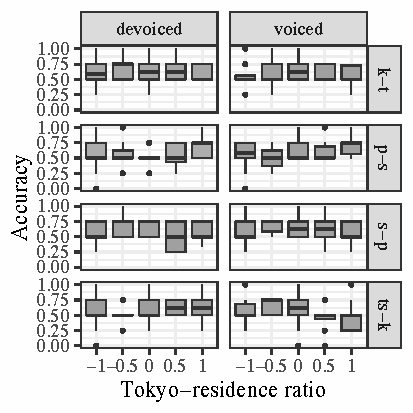
\includegraphics[width=6.5cm]{../results/artifact/results_axb_allophone_gray.pdf}
% 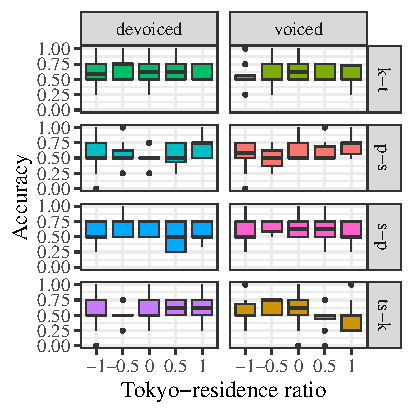
\includegraphics[width=6.5cm]{../results/artifact/results_axb_allophone.pdf}
\caption{A boxplot that shows the relationship between residential history and response accuracy.}\label{fig:axb_results}
\end{center}
\end{figure}

We checked the distribution of the reaction time data, and excluded 0.61\% of data with a reaction time of 10 seconds or longer as outliers. We calculated the mean accuracy, averaging four patterns based on the X in AXB (VC$_\text{1}$VC$_\text{2}$V or VC$_\text{1}$C$_\text{2}$V) and the correct answer position (A or B), and excluded missing values.

% FIXME: add table
We created a Bayesian linear mixed-effects model \cite{lme4, rstanarm, easystats} with the Tokyo--Kansai ratio as the independent variable, and the AXB task discrimination accuracy as the dependent variable. Items and participants were modeled as random effects. The analysis revealed an overall mean accuracy of 0.59, without consistent effects for environmental differences. The estimates of dialectal differences were positive (0.019), and not in the direction of decreasing precision.

To evaluate the null hypothesis, we calculated a Bayes factor ($BF$) for the Tokyo--Kansai ratio. The Bayes factor, which is used to compare the models in the framework of Bayesian statistics, was 0.150 and provided substantial evidence for the null hypothesis. In this study, we calculated the $BF$ as $Posterior \text{ }Odds / Prior \text{ }Odds$, where each $Odds$ is calculated as $P(b\notin[0, \infty] | Data)/P(b\in[0, \infty] | Data)$ and $P(b\notin[0, \infty])/P(b\in[0, \infty])$, respectively. Given that $b$, the estimates of the Tokyo--Kansai ratio, was supposed to be negative, the null region \cite{kruschke2010believe}, considered to have no effect, was set to a positive value [0, $\infty$].

The $BF$ of the Tokyo--Kansai ratio was 0.15, which indicated that the null hypothesis of a positive effect was $1/0.15(=6.67)$ times more plausible than the alternative hypothesis. This result contradicts the interpretation that the allophone increases the rate of illusions, and decreases its accuracy. All data and script are available at the corresponding author's repository https://github.com/kishiyamat/icphs2023~.

\subsection{2.3. Discussion}

If these allophones trigger the perceptual epenthesis, Tokyo dialect speakers should have lower accuracy in the discrimination experiment, than those without devoicing. However, the results of the AXB task showed that the discrimination accuracy of both Kansai and Tokyo dialect speakers, regardless of their language experience, was around 0.59, which is close to a chance level. In addition, the $BF$ suggested that the language experience and devoicing did not affect the rate of illusions in the discrimination task.

Furthermore, we examined whether dialect differences in language experience affect the offline goodness rating of deletion/devoicing. Note that we performed this categorization task after the online process, to avoid any effect on the validation of the online process.

\section{Categorization task}

\subsection{3.1. Materials and methods}

The participants in the perceptual task also completed the categorization task. All sounds presented in the perceptual task were categorized and rated. There were eight different patterns: four that were devoiced in the Tokyo dialect (esupo, ekuto, epuso, etsuko) and four that were not devoiced (ezubo, egudo, ebuzo, edzugo). Each of them had a devoiced counterpart, and the choices were shown in Japanese letters on the screen. Because three speakers recorded 16 patterns, the participants listened to 48 stimuli, selected one of the above eight options above that was closest to them, and rated its acceptability on a 7-point scale (0--6). In the rating, zero was considered "not appropriate at all," and six was considered "completely appropriate."

\subsection{3.2. Results}

% FIXME: make the figure gray-scale
% FIXME: check left/right panes
The $x$-axis in Figure \ref{fig:cat_results} shows the Tokyo--Kansai ratio, and the $y$-axis shows the goodness of fit rating. The left and right panes indicate the environment of speech (devoicing or not), and the color difference shows whether the actual stimulus was devoiced or not. The overall ratings were above the mean of 4. The devoiced stimuli were rated higher in the devoiced environment (left pane), while they were rated lower in the no-devoicing environment (right pane). The residential history did not contribute to these differences.
\begin{figure}[!ht]
\begin{center}
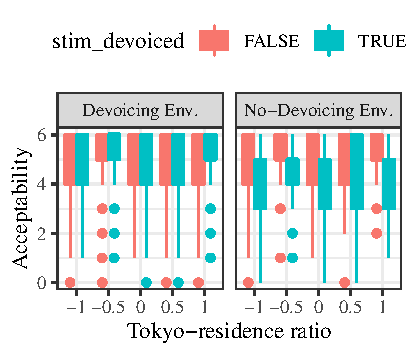
\includegraphics[width=6.5cm]{../results/artifact/results_categorization.pdf}
\caption{A boxplot that shows the relationship between the residential history and the goodness of fit rating.}\label{fig:cat_results}
\end{center}
\end{figure}

To test these points, we created a Bayesian linear mixed-effects model, with the goodness of fit rating as the dependent variable. The independent variables were environment (devoicing/no-devoicing), stimulus type (devoiced/not devoiced), the Tokyo--Kansai ratio, and their interactions. Participants and items were random effects, and we employed a normal distribution ($M=0$, $SD=10$), as a prior distribution for each parameter.

The mean rating was 4.87, indicating that the evaluation was generally natural, given that the rating range was 0--6. The estimates of the devoicing environment and the devoiced stimulus were $-0.37$ and $-0.79$, respectively. Furthermore, the interaction, that is, the devoiced stimulus in the devoiced environment, increased the rating by 1.19. The $BF$ for the Tokyo--Kansai ratio was 0.012 when the null region was set to $[-\infty, 0]$, indicating very strong evidence for the null hypothesis.

\subsection{3.3. Discussion}

The results showed that the overall responses were above 4, which means that the quality of the stimuli in this study was not lower than those in previous studies \cite{kilpatrick2018japanese}. If the participants can judge the devoiced speech in the Tokyo dialect offline without epenthesis, the rate of devoiced stimuli in a no-devoicing environment would be less than three. Considering the results of the categorization task, both the Tokyo and Kansai dialect speakers showed the increased rating when the speech was devoiced in a devoicing environment, while it decreased when the devoiced stimuli were in a no-devoicing environment. However, the interaction's $b$ was 1.19, and not high enough to cross the threshold between unnatural and natural.

\section{General Discussion}

Previous research proposed that devoicing could cause the perceptual epenthesis. In addition, probabilistic models included the distribution of auditory realizations. This study proposes two different interpretations, based on the results of perceptual experiments and categorization tasks.

First, the results of the discrimination accuracy and categorization tasks in the previous studies might not be due to the effect of devoicing, but because of acoustic differences. If the perceptual epenthesis were due to the devoicing or deletion, the discrimination accuracy of the Tokyo dialect speakers would be lower than that of the Kansai dialect speakers, who do not devoice or delete the vowels. However, no such effect was observed. Instead, Kansai dialect speakers perceived the illusory vowels almost the same as the Tokyo dialect speakers, in our study.

Second, regarding how acoustic cues affect speech perception, previous studies \cite{feldman2009influence, wilson2013bayesian, kishiyama2021influence} have assumed Eq. (\ref{hmm}) during inference. On the right-hand side, $P(S_{\text{new}}|c)$ is thought to represent the distribution of auditory realizations for phonemes or the perceptual likelihood of $S_{\text{new}}$ given $c$, and it does not need to be a generative model. This makes the results consistent with the previous study, because $P$( [\textsubring{\textturnm}] | /u/ ) or $P$( [s] | /su/ ) is not zero, given that the Kinki dialect speakers hear them in Tokyo dialect, which is prevalent in Japan. Given the Bayes' Theorem, the equation can be rewritten as
%
% \begin{equation} \label{disc}
%     \hat{c} = \argmax_{c} P(c | c_{t-1}) \frac{P(c|S_{\text{new}})}{P(c)},
% \end{equation}
%
$\hat{c} = \argmax_{c} P(c | c_{t-1}) P(c|S_{\text{new}}) / P(c)$,
and it integrates discriminative models instead of generative models. This allows us to employ other discriminative models, such as neural networks and multinomial logistic regressions. Given that previous studies have already supported the validity of HMMs \cite{kishiyama2021influence, kishiyama2022onestep}, we will test whether we can incorporate the above discriminative model into HMMs to explain behavioral data, in future studies.

% FIXME
\section{Acknowledgements}

This work was supported by JSPS KAKENHI Grant Numbers 20H01254 and 21K20027.

\bibliographystyle{IEEEtran}

\bibliography{mybib}

\end{document}

